\subsection{Markov Decision Process}\label{section:markov}

Markov decision process is a slightly advanced version of the Markov Chain. It includes action on top of the Markov Chain. Reinforcement learning problems are formalized as a Markov Decision Process rather than Markov Chain because RL agents are free to choose from different actions.

MDPs first came into play as part of the optimal control problem by Bellman \cite{Bellman1958}. Bellman applied dynamic programming methods to solve the MDP problem optimally. However, this methodology was not scalable to larger problems stemming from the curse of dimensionality problem \cite{Sutton2018}.

The fundamental elements of MDP are as follows:
\begin{itemize}
    \item Agent:  The actor takes an action in the environment to learn.
    \item Environment: The agent interacts with the Environment (Plant).
    \item Rewards: Environment returns rewards based on the interaction made by the actor.
    \item State: View of the environment from the eyes of the actor. 
\end{itemize}

\begin{figure}[htbp]
    \centering
    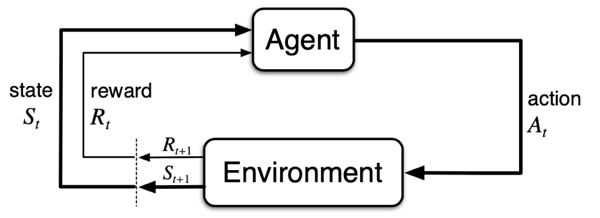
\includegraphics[width=0.8\textwidth]{figures/mdp}
    \caption{MDP structure}
    \label{fig: mdp}
\end{figure}

The action process follows; the agent acts on the environment at time t, and the environment returns the reward and state of the action at time \(t+1\). Based on the state of the environment at the \(t+1\) agent makes another action \(A_{t+1}\), which results in \(R_{t+2}\) and \(S_{t+2}\).

In every MDP system, agents should be reachable to every other states through a sequence of actions. The transition between states is of great value for the MDP framework.
One can compute the transition probability in MDP, given the inner dynamics of the environment \cite{Sutton2018}. The below equation defines the internal dynamics probability. It tells how probable it is to end up in state \(s'\) with reward \(r\) by taking action \(a\) in state \(s\). 

\begin{equation}
    p(s',r | s,a) = Pr\{S_t = s', R_t = r | S_{t-1} = d, A_{t-1} = a\}
\end{equation}

One can calculate the transition probability function from the inner dynamics' probability function.

\begin{equation}
    p(s'|s,a) = Pr\{S_t=s'| S_{t-1}=s, A_{t-1}=a\} = \sum_{r \in R}p(s',r|s,a)
\end{equation}

Next chapter, we will dive into the definition of the reward and value function. Based on those concepts, we will build the logic on how to solve MDPs optimally.